\chapter{Markov chain Monte Carlo (MCMC)}
\label{ch:mcmc}

As seen from the previous part, many-body systems exhibit a rich variety of physical phenomena emerged from statistics of microscopic configurations. Their exponentially large configuration spaces prohibit us from evaluating observables by exact enumerations, and motivate us to use numerical approximation methods in the studies of their properties. In this part, we focus on such techniques for classical systems, which are relatively simpler than quantum ones. We first review the traditional method of Markov chain Monte Carlo (MCMC) and the variational method, list some commonly used ansatzes to approximate the Boltzmann distribution, and discuss their limitations. Then we introduce the autoregressive models with the advantage of exact sampling, and combine the strengths of the exact sampling and the Markov chain sampling to remove the bias in the variational method.

\section{Monte Carlo method}
\label{sec:monte-carlo}

When studying an observable of a classical many-body system in \cref{eq:cl-obs}, we have seen that it consists of a summation over all configurations of the system, which costs an exponentially large amount of computation if performed by an exact enumeration. Instead, to obtain the result within a practical computation budget, a general method is to generate many random samples of configuration $\{\vs^{(1)}, \vs^{(2)}, \ldots, \vs^{(M)}\}$ following the target distribution $p(\vs)$, where $M$ is the sample size, then estimate the $p$-weighted summation over all configurations by the uniform average over only the samples:
\begin{equation}
\bbE_\text{MC}[O] = \frac{1}{M} \sum_{i = 1}^M O\left( \vs^{(i)} \right).
\label{eq:monte-carlo}
\end{equation}
This method is named Monte Carlo, after the casino that would later become famous to every computational physicist~\cite{metropolis1949monte, landau2021guide1}. It is proven that~\cite{feller1968extention}
\begin{equation}
\Var\big[ \bbE_\text{MC}[O] \big] = \frac{1}{M} \Var[\bar{O}],
\label{eq:monte-carlo-var}
\end{equation}
where the sample variance $\Var\big[ \bbE_\text{MC}[O] \big] = \bbE_\text{MC}\left[ \left( O - \bbE_\text{MC}[O] \right)^2 \right]$ and the true variance $\Var[\bar{O}] = \overline{(O - \bar{O})^2}$. Therefore, the sample variance vanishes and the estimator converges to the true value as $M$ increases, given that the true variance is finite, and all samples are independently drawn from the true distribution.

\section{Exact sampling}

The Monte Carlo method requires randomly generating independent samples from a given distribution, but this is not always straightforward. In computational physics, the so-called ``random numbers'' are produced by pseudorandom number generators (PRNG)~\cite{press2007numerical}, which are originally designed to generate statistically random values from the univariate uniform distribution $\calU$ over an interval, such as $[0, 1)$. In some simple cases, we can transform every sample from the PRNG to the target distribution in a deterministic way: Univariate distributions can be sampled by a change of variable, also known as reparameterization. For example, the exponential distribution $p(x) = \rme^{-x}$, $x \in [0, +\infty)$ can be sampled by $x = -\ln u$, where $u$ is randomly generated from $\calU[0, 1)$, as the probability density function (PDF) satisfies
\begin{equation}
p(x) = q(u) \left| \frac{\partial u}{\partial x} \right| = 1 \cdot \left| \frac{\partial}{\partial x} \rme^{-x} \right| = \rme^{-x}.
\end{equation}
Multivariate distributions can be sampled by first generating multiple independent values from $\calU[0, 1)$ and then changing the variables. For example, the 2D unit Gaussian distribution
$p(x, y) = \frac{1}{2 \pi} \rme^{-\frac{1}{2} (x^2 + y^2)}$ can be sampled by the Box--Muller transform~\cite{box1958note}:
\begin{gather}
p(x, y) = q(u) q(v) \begin{Vmatrix}
\frac{\partial u}{\partial x} & \frac{\partial u}{\partial y} \\
\frac{\partial v}{\partial x} & \frac{\partial v}{\partial y}
\end{Vmatrix}, \label{eq:reparam} \\
x = r \cos \theta, \quad y = r \sin \theta, \\
r = \sqrt{-2 \ln u}, \quad \theta = 2 \pi v,
\end{gather}
where $u$ and $v$ are independently sampled from $\calU[0, 1)$, and $\lVert \cdot \rVert$ denotes the absolute value of the determinant of the matrix. Discrete distributions can be obtained by discretizing continuous distributions. For example, the Bernoulli distribution $p(x) = (1 - p_1) \delta_{x, 0} + p_1 \delta_{x, 1}$ with the parameter $p_1 \in [0, 1]$ can be sampled by \cref{alg:bernoulli}. In this thesis, we refer to this kind of sampling methods as exact sampling.

\begin{algorithm}[H]
\caption[Discrete Bernoulli distribution from continuous uniform distribution]{
Discrete Bernoulli distribution from continuous uniform distribution.
}
\label{alg:bernoulli}
\begin{algorithmic}[1]
\STATE Sample $u$ from $\calU[0, 1)$
\IF{$u < p_1$}
    \STATE Output $x = 0$, $p(x) = 1 - p_1$
\ELSE
    \STATE Output $x = 1$, $p(x) = p_1$
\ENDIF
\end{algorithmic}
\end{algorithm}

\section{Markov chain sampling}

In the case of Boltzmann distributions for many-body systems with complicated energy landscapes, an analytical transformation for exact sampling is generally impossible to find, and we can only resort to indirect methods for sampling these distributions. A common method is to construct a Markov chain of samples, whose equilibrium distribution converges to the target one, therefore this sampling method is known as Markov chain Monte Carlo (MCMC)~\cite{gelfand1990sampling, robert2020markov}. For spin systems, such a Markov chain is usually constructed by the Metropolis--Hastings algorithm~\cite{hastings1970monte}. In each sampling step, we propose to update the current configuration $\vs$ to a new one $\vs'$ with the proposal distribution $g(\vs' \mid \vs)$, where $\sum_{\vs'} g(\vs' \mid \vs) = 1$ for all $\vs$. Then we accept $\vs'$ to become the current configuration by an acceptance probability\footnote{The acceptance probability depends on the configurations $\vs$ and $\vs'$, not to be confused with the acceptance rate defined over the whole Markov chain.} defined by
\begin{equation}
A(\vs \to \vs') = \min\left( 1, \frac{p(\vs') g(\vs \mid \vs')}{p(\vs) g(\vs' \mid \vs)} \right).
\label{eq:metropolis}
\end{equation}
Otherwise, we reject it and rollback to $\vs$. It can be checked that the target distribution $p(\vs)$ is exactly an equilibrium distribution of the Markov transition matrix:
\begin{gather}
M_{\vs_j \vs_i} = A(\vs_i \to \vs_j) g(\vs_j \mid \vs_i), \label{eq:markov-matrix} \\
\sum_{\vs_i} M_{\vs_j \vs_i} p(\vs_i) = p(\vs_j).
\end{gather}
If we want to sample the target distribution using a single Markov chain, i.e., the target distribution is the only equilibrium distribution, then the proposals must be ergodic, which allows the initial configuration to transition to all configurations in a finite number of samples. The simplest method to propose an update is to randomly select a spin and flip it, therefore $g(\vs' \mid \vs) = g(\vs \mid \vs')$ for all $\vs$ and $\vs'$, and \cref{eq:metropolis} simplifies to
\begin{equation}
A(\vs \to \vs') = \min\left( 1, \frac{p(\vs')}{p(\vs)} \right).
\end{equation}
More advanced choices of $g(\vs' \mid \vs)$ will be discussed in \cref{sec:more-sampling}.

When $p(\vs)$ is the Boltzmann distribution in \cref{eq:boltzmann}, the acceptance probability further simplifies to
\begin{equation}
A(\vs \to \vs') = \min\left( 1, \rme^{\,\beta \left( H(\vs) - H(\vs') \right)} \right).
\end{equation}
It avoids computing the partition function $Z$, which consists of a summation over exponentially many configurations. In the case of locally interacting systems, such as \cref{eq:cl-ising-nnn}, the energy difference of flipping a spin $s_i$ simplifies to
\begin{equation}
H(\vs) - H(\vs') = 2 s_i \left( \sum_{\text{$j$ that interacts with $i$}} J_{i j} s_j \right),
\end{equation}
so the time to compute the acceptance probability, and therefore the total time of a sampling step to propose and accept a sample, only depends on the number of neighbors interacting with a site, rather than the whole system size. This advantage makes MCMC a feasible method to study large systems.

After collecting many samples from the Markov chain, we estimate the observables using \cref{eq:monte-carlo}. Care should be taken when generating these samples, as we will discuss in the following.

\section{Autocorrelation time}
\label{sec:iat}

\subsection{Autocorrelation in Markov chain}

\begin{figure}[htb]
\centering
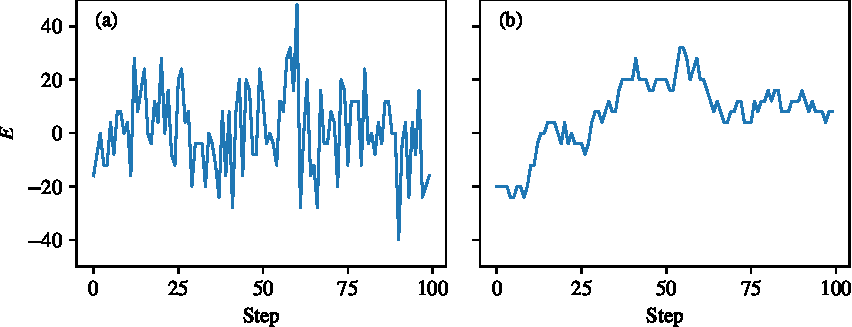
\includegraphics[width=\linewidth]{ch3/rand_autocorr.pdf}
\caption[Energy of Ising model from independent and autocorrelated samples]{
Energies of $100$ samples for the Ising model on the $10 \times 10$ square lattice.
(a) The samples are independently generated from the uniform distribution.
(b) The samples are generated by single-spin updates with $\beta = 0$, thus have autocorrelation.
}
\label{fig:rand-autocorr}
\end{figure}

Although MCMC allows us to estimate the observables from complicated distributions where an exact sampling method cannot be easily constructed, it breaks the assumption of \cref{eq:monte-carlo} that the samples should be independent. In each sampling step, we propose a new configuration $\vs'$ that depends on the current configuration $\vs$, such as flipping a single spin. Moreover, we may reject $\vs'$ and keep using $\vs$ to evaluate the observable for this step. The visual difference between a sequence of independent samples and a Markov chain is shown in \cref{fig:rand-autocorr}. Quantitatively, the samples in the Markov chain $\{\vs^{(1)}, \vs^{(2)}, \ldots, \vs^{(M)}\}$ produce autocorrelation in the observable values~\cite{muller1973dynamic}:
\begin{equation}
C_{O, M}(t) = \left( \frac{1}{M - t} \sum_{i = 1}^{M - t} O\left( \vs^{(i)} \right) O\left( \vs^{(i + t)} \right) \right) - \bbE_\text{MCMC}^2[O],
\end{equation}
where $\bbE_\text{MCMC}[O]$ has the same form as \cref{eq:monte-carlo}, but uses the samples from the Markov chain. We mainly consider the large sample size limit
\begin{equation}
C_O(t) = \lim_{M \to \infty} C_{O, M}(t).
\end{equation}
The correlated samples cause $C_O(t) \neq 0$ when $t > 0$. For example, \cref{fig:autocorr} shows the autocorrelation in energy $C_E(t)$ of the $10 \times 10$ Ising model. As the number of steps $t$ between two samples increases, the average autocorrelation between the two samples decays to zero. At the critical point $\beta_\text{c} = \frac{1}{2} \ln(1 + \sqrt{2}) \approx 0.44$~\cite{onsager1944crystal}, the autocorrelation decays particularly slowly, and we can assume that a sample is approximately independent of the original one only after as many as $10^4$ steps, which renders the MCMC sampling inefficient.

\begin{figure}[htb]
\centering
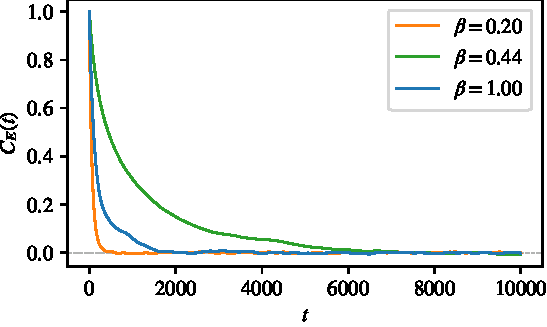
\includegraphics[width=0.7\linewidth]{ch3/autocorr.pdf}
\caption[Autocorrelation in energy for Ising model at different temperatures]{
Autocorrelation in energy $C_E(t)$ of the Ising model on the $10 \times 10$ square lattice at different inverse temperatures $\beta$. The samples are generated by single-spin updates, and the autocorrelation is estimated using $10^7$ samples.
}
\label{fig:autocorr}
\end{figure}

\subsection{Integrated autocorrelation time}

The integrated autocorrelation time~\cite{ambegaokar2010estimating, goodman2010ensemble}, or ``autocorrelation time'' for short, is a metric for MCMC to assess the loss in sample diversity due to autocorrelation, defined by
\begin{align}
\tau = \sum_{t = 1}^\infty r_O(t), \label{eq:iat} \\
r_O(t) = \frac{C_O(t)}{C_O(0)}, \label{eq:rt}
\end{align}
where $r_O(t)$ is the normalized autocorrelation. The value of $\tau$ depends on the complexity of the target distribution, and the method to propose new configurations. It is also known as the relaxation time in analytical studies of the spin dynamics. When estimating it in practice, $C_O(t)$ is replaced by $C_{O, M}(t)$ with a sufficiently large chain length $M$, and we need to verify $M \gg \tau$ after obtaining $\tau$. The summation $\sum_{t = 1}^\infty$ is also replaced by a finite summation $\sum_{t = 1}^{t_\text{cutoff}}$, where $t_\text{cutoff}$ is the first step when $C_{O, M}(t)$ crosses zero~\cite{wu2021unbiased}. It can be efficiently computed using fast Fourier transform (FFT) by the Wiener--Khinchin theorem~\cite{wiener1930generalized}. Other methods to estimate $\tau$ include binning analysis~\cite{wallerberger2018efficient}, and fitting the exponential decay of $C_O(t)$~\cite{bialas2023analysis}. These methods should produce consistent results when the chain length $M$ is sufficiently large.

\begin{figure}[htb]
\centering
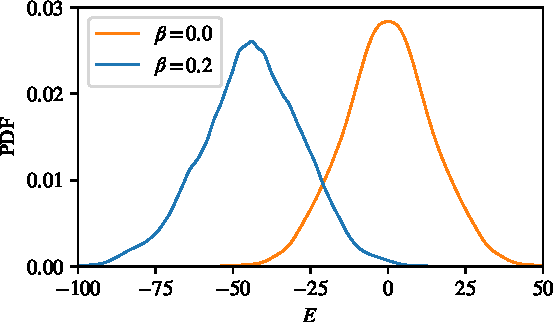
\includegraphics[width=0.7\linewidth]{ch3/energy_hist.pdf}
\caption[Distribution of energy for Ising model at different temperatures]{
Distribution of energy $E$ for the Ising model on the $10 \times 10$ square lattice at inverse temperatures $\beta = 0$ (uniform distribution) and $0.2$ (Boltzmann distribution with moderately high temperature).
The typical energies from the two distributions differ by approximately $50$, and for larger systems and lower temperatures the difference will be even larger, which leads to exponentially low acceptance probability.
The probability density function (PDF) of the distribution is estimated from the samples using Silverman’s method~\cite{silverman1986density}.
}
\label{fig:energy-hist}
\end{figure}

Intuitively, the autocorrelation time takes two factors into account that affect the sample diversity: the correlation between the proposed configuration and the current one, and the acceptance probability. For single-spin updates, the successive samples are almost fully correlated, which leads to high autocorrelation in the observable values. On the other extreme, if we do global updates, i.e., randomly generate a proposed configuration $\vs'$ from the uniform distribution of all configurations in each sampling step, then it is fully uncorrelated with the current one. However, the energy $H(\vs')$ from the uniform distribution is almost always much higher than the current one from the target distribution, as shown in \cref{fig:energy-hist}, which makes the acceptance probability exponentially low, and the collected samples are still almost fully correlated. Between the two extremes of single-spin updates and global updates, a variety of cluster updates have been proposed to balance these two factors, which we will discuss in \cref{sec:cluster-update}.

\subsection{Effective sample size}

The loss in sample diversity is reflected quantitatively in the variance of the Monte Carlo estimator in \cref{eq:monte-carlo-var}. When the Markov chain is in equilibrium, in the presence of autocorrelation, the variance increases to
\begin{equation}
\Var\big[ \bbE_\text{MCMC}[O] \big] = \frac{1}{M_{\text{eff}\,\tau}} \Var[\bar{O}],
\end{equation}
where the effective sample size
\begin{equation}
M_{\text{eff}\,\tau} = \frac{1}{2 \tau + 1} M
\label{eq:eff-sample-size}
\end{equation}
is less than the original sample size $M$.

\section{Critical slowing down}
\label{sec:critical-slow}

\begin{figure}[htb]
\centering
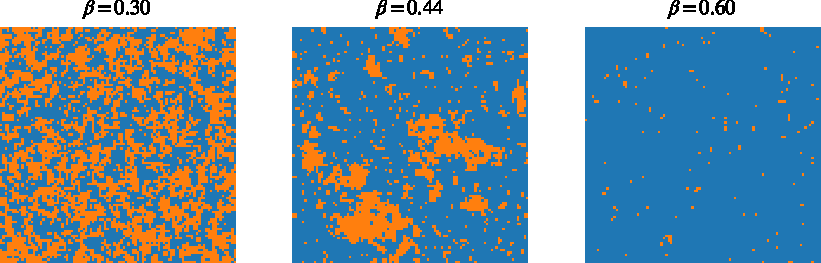
\includegraphics[width=\linewidth]{ch3/ising_samples.pdf}
\caption[Sample of Ising model at different temperatures]{
A typical sample of the Ising model on the $100 \times 100$ square lattice at different inverse temperatures. The blue and the orange plaquettes denote spin up and down respectively. Around the critical point $\beta_\text{c} \approx 0.44$, the clusters of spins are particularly visible, which pose difficulty to MCMC with single-spin updates.
}
\label{fig:ising-samples}
\end{figure}

In many-body systems, the autocorrelation time particularly depends on the physical parameters, such as the inverse temperature $\beta$. It is a long-standing issue with MCMC that the autocorrelation time significantly increases when the system is around its critical point, known as the critical slowing down~\cite{goodman1989multigrid, wolff1990critical}. Intuitively, the collective dynamics of the spins form clusters in the system, which separate from each other by domain walls, as shown in \cref{fig:ising-samples}. Their average diameter is roughly the correlation length $\xi$ of the system. In the case of single-spin update, the Markov chain can be interpreted as a random walk in the configuration space, where it moves from one configuration to an adjacent one with a spin flipped. As a corollary, the time $\tau$ to walk the distance $\xi$ scales by $\tau \sim \xi^2$, regardless of the spatial dimension. Detailed analysis from lattice field theory has shown that $\tau \sim \xi^z$, where $z$ is the dynamical critical exponent, and $z \approx 2$ in many cases~\cite{hohenberg1977theory}. At the critical point, $\xi$ diverges until it is bounded by the system size~\cite{lubetzky2012critical}, therefore the critical slowing down occurs.

From the perspective of statistical complexity~\cite{lopez1995statistical}, the Boltzmann distribution at the critical temperature is hard to sample from because it has both low entropy and uniformity, which lead to high complexity. It is between the high-temperature distribution with low uniformity but high entropy, and the low-temperature distribution with low entropy but high uniformity. This phenomenon proposes challenge to studies of phase transitions using MCMC, and can be alleviated by cluster updates.

\section{Burn-in stage and Gelman--Rubin statistic}

The autocorrelation time $\tau$ is a crucial metric for the efficiency of an MCMC algorithm when the Markov chain is already in equilibrium. However, at the beginning of MCMC, the configuration is usually initialized ``randomly'', which is from the uniform distribution of all configurations. The Markov chain can take many steps to transition from the initial configuration to a typical one in the target distribution, and these steps are called the burn-in or warm-up stage. The untypical samples in this stage introduce bias in the estimation of observables, unless we have exponentially many samples in total to compensate the exponentially low probabilities of untypical samples. To avoid this bias, we discard these samples and start collecting actual samples after this stage.

In theory, the length of the burn-in stage is at most on the order of magnitude of $\tau$, which lets the new configuration decorrelate with the initial one, but in practice we can estimate $\tau$ only if we already know that the burn-in stage has ended. Therefore, we need another metric to estimate the length of the burn-in stage before collecting samples from the equilibrium distribution, which can only be derived from dynamical properties of the Markov chain.

\begin{figure}[htb]
\centering
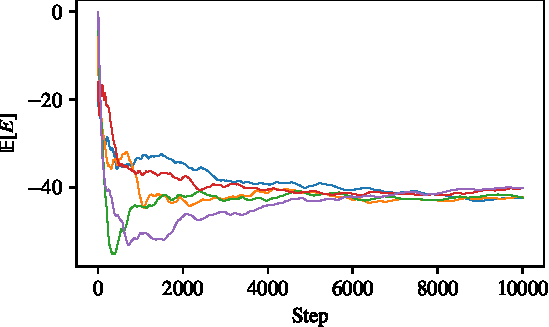
\includegraphics[width=0.7\linewidth]{ch3/multi_chains.pdf}
\caption[Convergence of multiple Markov chains]{
Convergence of five different Markov chains, shown with different colors, for the Ising model on the $10 \times 10$ square lattice at inverse temperature $\beta = 0.2$.
The $y$-axis is the estimated energy using the samples up to the current step.
Although the chains start from different random initializations, they eventually reach the equilibrium distribution and produce consistent estimations of the energy after sufficiently many steps.
}
\label{fig:multi-chains}
\end{figure}

The Gelman--Rubin (GR) statistic~\cite{gelman1992inference, vats2021revisiting} can be used to identify whether the Markov chain has reached the equilibrium. To compute the GR statistic, we generate multiple independent Markov chains starting from different random initial configurations, as shown in \cref{fig:multi-chains}, which is already a common practice to utilize the parallelization capability of modern computers~\cite{lee2010utility}. The samples are denoted by $\vs^{(j, m)}$, where $j \in [1, J]$ identifies the chain and $m \in [1, M]$ identifies the sampling step, and the corresponding observable values are denoted by $O_{j, m} = O\left( \vs^{(j, m)} \right)$. Then we have
\begin{align}
\bar{O}_j &= \frac{1}{M} \sum_{m = 1}^M O_{j, m}, \\
\bar{O}_* &= \frac{1}{J} \sum_{j = 1}^J \bar{O}_j, \\
s^2_j &= \frac{1}{M - 1} \sum_{m = 1}^M (O_{j, m} - \bar{O}_j)^2, \\
s^2_* &= \frac{1}{J} \sum_{j = 1}^J W_j,
\end{align}
where $\bar{O}_j$ is the sample mean of the observable over a chain, $\bar{O}_*$ is the sample mean of all chains, $s^2_j$ is the sample variance of a chain, and $s^2_*$ is the mean of these sample variances. Due to the presence of autocorrelation, each $s^2_j$ underestimates the true variance of the target distribution $\sigma^2$. A correction to this bias is estimated by comparing the means of different chains:
\begin{equation}
\frac{B}{M} = \frac{1}{J - 1} \sum_{j = 1}^J (\bar{O}_j - \bar{O}_*)^2.
\end{equation}
Now the estimated variance is
\begin{equation}
\sigma^2_* = \frac{M - 1}{M} s^2_* + \frac{B}{M}.
\end{equation}
The GR statistic is defined to normalize the correction to the estimated variance:
\begin{equation}
R = \sqrt{\frac{\sigma^2_*}{s^2_*}}.
\end{equation}
It is also related to the effective sample size by
\begin{equation}
R \approx \sqrt{1 + \frac{M}{M_\text{eff}}}.
\end{equation}
If we have enough random Markov chains from different initial configurations, which cover all regions of interest in the configuration space, and converge to similar distributions with mean observable values close to each other, then we can assume that the Markov chains have reached equilibrium. It was originally proposed in Ref.~\cite{gelman1992inference} to use a threshold $R < \delta$, and a common choice is $\delta = 1.1$. According to Ref.~\cite{vats2021revisiting}, practical choices of $\delta$ ranges from $1.003$ to $1.3$, and a more stable estimation of the true variance can be obtained from batch-wise variances in the chains.

\section{Other sampling methods}
\label{sec:more-sampling}

\subsection{Importance sampling}
\label{sec:importance-sampling}

Apart from the exact sampling and the MCMC sampling, there are other sampling methods to estimate the observable in \cref{eq:cl-obs}. In principle, we can generate samples $\{\vs^{(1)}, \vs^{(2)}, \ldots, \vs^{(M)}\}$ from any distribution $q(\vs)$, then estimate the observable by
\begin{align}
\bbE_\text{imp}[O] &= \frac{\sum_{i = 1}^M w\left( \vs^{(i)} \right) O\left( \vs^{(i)} \right)}{\sum_{i = 1}^M w\left( \vs^{(i)} \right)}, \label{eq:importance-sampling} \\
w\left( \vs^{(i)} \right) &= \frac{p\left( \vs^{(i)} \right)}{q\left(\vs^{(i)} \right)},
\end{align}
given that $q(\vs)$ has a wider support than $p(\vs)$, i.e., $q(\vs) > 0$ for all $\vs$ such that $p(\vs) > 0$. The probabilities $p(\vs)$ and $q(\vs)$ can be unnormalized, as an overall coefficient in $w(\vs)$ will cancel out in the numerator and the denominator of $\bbE_\text{imp}[O]$. This method is called importance sampling in statistics~\cite{kloek1978bayesian, bugallo2017adaptive}, and the distribution $q(\vs)$ is called an ansatz\footnote{The word ``ansatz'' is borrowed from German. Its plural form is ``Ansätze'' in German, but the adapted form ``ansatzes'' is also used in English literature.} in the context of statistical physics. The ansatz should be close to $p(\vs)$, and easier to sample from than $p(\vs)$. Some choices of the ansatz for importance sampling will be discussed in \cref{sec:nmf}. The variance of this estimator is
\begin{equation}
\Var\big[ \bbE_\text{imp}[O] \big] = \frac{1}{M_{\text{eff}\,w}} \Var[\bar{O}],
\label{eq:importance-sampling-var}
\end{equation}
where the effective sample size
\begin{equation}
M_{\text{eff}\,w} = \frac{\Big( \sum_{i = 1}^M w\left( \vs^{(i)} \right) \Big)^2}{\sum_{i = 1}^M w^2\left( \vs^{(i)} \right)}.
\label{eq:eff-sample-size-w}
\end{equation}
The variance reaches its minimum when $q(\vs) = p(\vs)$, which is in accordance with the intuition that $q(\vs)$ should be as close to $p(\vs)$ as possible.

\subsection{MCMC importance sampling}

Besides reweighing the samples from $q(\vs)$ using the target distribution $p(\vs)$, we can also use the Metropolis--Hastings algorithm in \cref{eq:metropolis} to reject the samples, which we refer to as MCMC importance sampling~\cite{liesenfeld2008improving, schuster2020markov}. In each sampling step, we propose a new configuration $\vs'$ from the distribution $q(\vs')$, which is independent of the current configuration $\vs$, i.e., the proposal distribution $g(\vs' \mid \vs) = q(\vs')$. Then the acceptance probability becomes
\begin{equation}
A(\vs \to \vs') = \min\left( 1, \frac{p(\vs') q(\vs)}{p(\vs) q(\vs')} \right),
\label{eq:mcmc-importance}
\end{equation}
which is close to $1$ if $q(\vs)$ is close to $p(\vs)$. Moreover, this method also reduces the correlation between $\vs$ and $\vs'$ compared to the single-spin update, which leads to the overall reduction of the autocorrelation time. An empirical comparison of the importance sampling and the MCMC importance sampling will be presented in \cref{sec:ncus}. More advanced methods have been proposed to construct the proposal distribution $g(\vs' \mid \vs)$ depending on the current configuration $\vs$, such as the Langevin Monte Carlo~\cite{rossky1978brownian} and the Hamiltonian Monte Carlo~\cite{duane1987hybrid}.

\subsection{Cluster update}
\label{sec:cluster-update}

A variety of cluster update algorithms can also be discussed in the framework of MCMC importance sampling. They have originally arisen from studies of the percolation transition in statistical physics and graph theory, or the series expansion of the partition function~\cite{fortuin1972random, leung1991percolation, evertz1993cluster}. A prominent example is the Wolff algorithm~\cite{wolff1989collective} for Ising models with two-body interactions. In each sampling step, it constructs and flips a cluster of spins according to \cref{alg:wolff}. The resulting proposal probability satisfies $g(\vs' \mid \vs) \propto p_\text{B}(\vs')$, so the acceptance probability is always $1$, which makes the Wolff cluster update far more efficient than the single-spin update when it is applicable.

\begin{algorithm}[H]
\caption[Wolff cluster update]{
Wolff cluster update algorithm to construct and flip a cluster of spins, in the MCMC sampling of the Boltzmann distribution of Ising models with two-body interactions.
$\calC$ is the cluster, $\calB$ is a set of spins on the boundary of the cluster, $\beta$ is the inverse temperature, $\partial i$ denotes the neighbors of the site $i$, and \texttt{rand()} generates a random number from the uniform distribution over $[0, 1)$.
}
\label{alg:wolff}
\begin{algorithmic}[1]
\STATE Input the current configuration $\vs$, interactions $\mJ$
\STATE Randomly choose a site $i$, $\calC \gets \{i\}$, $\calB \gets \{i\}$
\WHILE{$\calB \neq \emptyset$}
    \STATE $i \gets$ any site in $\calB$
    \FOR{$j \in \partial i$}
        \IF{$j \notin \calC$ \AND \texttt{rand()} $> \rme^{\,2 \beta J_{i j} s_i s_j}$}
            \STATE $\calC \gets \calC \cup \{j\}$, $\calB \gets \calB \cup \{j\}$
        \ENDIF
    \ENDFOR
    \STATE $\calB \gets \calB \setminus \{i\}$
\ENDWHILE
\FOR{$i \in \calC$}
    \STATE $s_i \gets -s_i$
\ENDFOR
\STATE Output the new configuration $\vs' \gets \vs$
\end{algorithmic}
\end{algorithm}

\dwcomment{Maybe discuss parallel tempering if there is spare time and space, but it's not used anywhere else in this thesis}

\section{Mode collapse}
\label{sec:mode-collapse}

Even if we collect effectively independent samples according to the autocorrelation time and the Gelman--Rubin statistic, it can still be questionable whether those samples actually represent the entire target distribution. The target distribution can have multiple modes, where a ``mode'' is defined to be a cluster of configurations $\{\vs_1, \vs_2, \vs_3, \ldots\}$ with high target probabilities $p(\vs_i)$ and high Markov transition probabilities $M_{\vs_j \vs_i}$ in \cref{eq:markov-matrix} between each other. The paths of configurations to transition from one mode to another always encounter energy barriers, whose heights are proportional to the system size, so the probability of visiting different modes is exponentially low. A possible failure of MCMC is the mode collapse, where the Markov chain is seemingly in equilibrium, but actually it is only in ``equilibrium'' within a single mode, and it takes an impractically long time to visit another mode, which leads to bias in the estimation of observables.

\begin{figure}[htb]
\centering
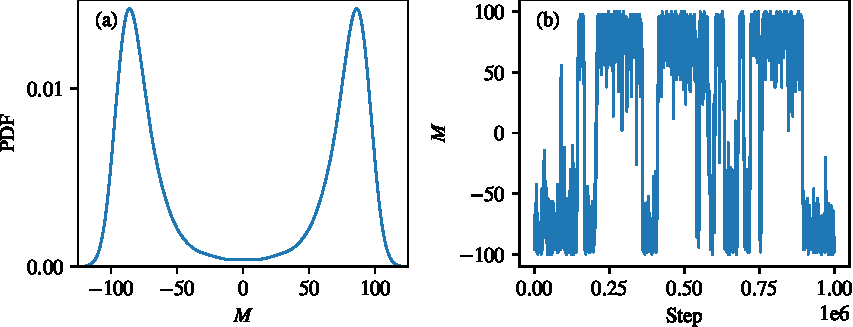
\includegraphics[width=\linewidth]{ch3/mag_hist.pdf}
\caption[Distribution and sampling of magnetization for Ising model]{
(a) Distribution of magnetization $M$ for the Ising model on the $10 \times 10$ square lattice at inverse temperature $\beta = 0.44$.
The two modes characterized by the magnetization are clearly visible.
The energy barrier between the two modes will be even higher as the system size increases, leading to exponentially low probability of transitioning from one mode to another.
The probability density function (PDF) of the distribution is estimated from the samples using Silverman’s method~\cite{silverman1986density}. \\
(b) Magnetizations of samples generated by single-spin updates. The Markov chain can stay in a mode for as long as $10^5$ steps before transitioning to another mode.
}
\label{fig:mag-hist}
\end{figure}

Intuitively, a mode is a peak of the target distribution in the configuration space. Although the exponentially high-dimensional configuration space is hard to visualize, we can characterize different modes by appropriate observables, such as the energy or the magnetization, and display the modes as peaks on the histogram of the observable. When the mode collapse happens, the estimated observable characterizing the uncovered modes becomes biased. A typical example is the two modes around the two degenerate ground states $\vs = (+1, +1, +1, \ldots)$ and $\vs = (-1, -1, -1, \ldots)$ in the ferromagnetic Ising model, as shown in \cref{fig:mag-hist}. In this case, even if the estimated energy is still close to the true value in a single mode, the magnetization becomes biased.

The mode collapse in the simple case above can be eliminated by applying the spin flipping symmetry to the generated samples. Other symmetries of the Hamiltonian, such as translations, rotations, and reflections, are also useful to alleviate the mode collapse and improve the accuracy of the estimated observables. Cluster updates are another approach to alleviate this problem, as they can propose large updates to the configuration to transition through the energy barriers that block local updates. The problem becomes more challenging in frustrated models, where the number of degenerate ground states can be exponentially large, and cannot be eliminated by a polynomially large symmetry group~\cite{wannier1950antiferromagnetism, mambrini1999residual, vanderstraeten2018residual}.

The effect of mode collapse is also demonstrated in the context of importance sampling in \cref{eq:importance-sampling}. Assuming the actual distribution of samples $q(\vs)$ only covers a single mode, and is exponentially suppressed in the uncovered modes, where $p(\vs) > 0$ but $q(\vs) \to 0$. Then we have pathologically high $w(\vs)$ in the uncovered modes, which cause the variance in \cref{eq:importance-sampling-var} to diverge. These configurations are identified as the exponentially suppressed configurations (ESC) in Ref.~\cite{wu2021unbiased}. Even if an estimated observable is still close to the true value in a single mode, the diverging variance indicates that such estimation is unreliable.

\begin{figure}[htb]
\centering
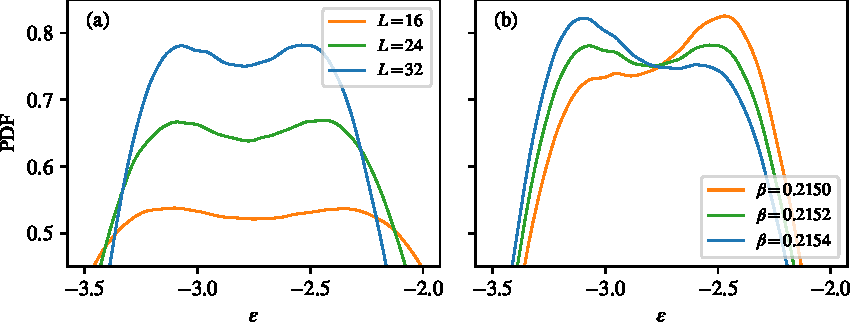
\includegraphics[width=\linewidth]{ch3/fpm_hist_p.pdf}
\caption[Distribution of energy for FPM with different sizes and temperatures]{
Distribution of the energy per site $E / N$ for the frustrated plaquette model (FPM) in \cref{sec:fpm}.
(a) The results with different system sizes, at their respective ``phase transition'' temperatures where the two peaks have the same area.
(b) The results at different temperatures, with the system size $L = 32$.
The probability density function (PDF) of the distribution is estimated from the samples using Silverman’s method~\cite{silverman1986density}.
The panel (a) is reproduced from Fig.~5 in Ref.~\cite{wu2021unbiased}.
}
\label{fig:fpm-hist-p}
\end{figure}

A particular consequence of mode collapse is the difficulty of MCMC sampling around first-order phase transitions of many-body systems. The first-order phase transition is characterized by a discontinuity in the energy. As an example, we investigate the transition between the ferrimagnetic (fM) and the paramagnetic (PM) phases in the 2D frustrated plaquette model (FPM) in \cref{sec:fpm}, with $N = L \times L$ spins. When we plot its distribution of energies in \cref{fig:fpm-hist-p}, we can see two peaks appearing around the transition temperature. As shown in the panel (a), the depth of the valley between the two peaks grows as the system size $L$ increases, which indicates an increasing energy barrier that blocks local updates. Compared to the peak on the left, the one on the right contains more excited states, but each has lower probability, so the areas of the two peaks are comparable. When the temperature increases, the low-energy peak shrinks while the high-energy one grows, as shown in the panel (b).

The first-order phase transition appears when the two peaks happen to have the same area. In the thermodynamic limit, the probability distribution is exponentially concentrated at the largest peak, so a change of the largest peak causes a discontinuity in the mean energy. Around the phase transition temperature, it is difficult for the system to reach thermal equilibrium, and the system can stay in a metastable state, or can be described by a superposition of multiple classical states. This two-peak distribution proposes challenge to MCMC with local updates, and cluster updates are a viable approach to this problem, as we will discuss in \cref{sec:ncus}.
